\graphicspath{{./figures/}}
\chapter{Implementation}
This chapter focuses on the overall project's implementation.
It mainly covers the four parts hardware assembly, long jump analysis,
drone control and their consolidation into one \ac{GUI}.

\section{Long-jump analysis software}\label{sec:4_analysis_software}
In order to analyze recorded long jump videos a ground station software is
developed.
Generally, the analysis is performed regarding the following set of
parameters:
\begin{itemize}
    \item left / right knee angle
    \item left / right arm angle
    \item takeoff angle
    \item left / right foot position
    \item hip height
\end{itemize}
These parameters are tracked over the whole jump, beginning with the run-up
throughout the takeoff until the landing.\\
\autoref{fig:4_long_jump_sketch} shows a detailed overview over the video data
that can be analyzed by the software.\\
As the takeoff is (one of) the most important phases in a long jump, it is
important to be able to detect the takeoff in a video.
Such a takeoff detection is developed alongside the above-mentioned parameter 
detection- and calculation.\\
This section will first introduce the body key point detection process that
is basis for all following calculations.
Afterwards, an algorithm for an automatic takeoff frame detection based on a
video input is implemented.
\begin{figure}[!h]
    \centering
    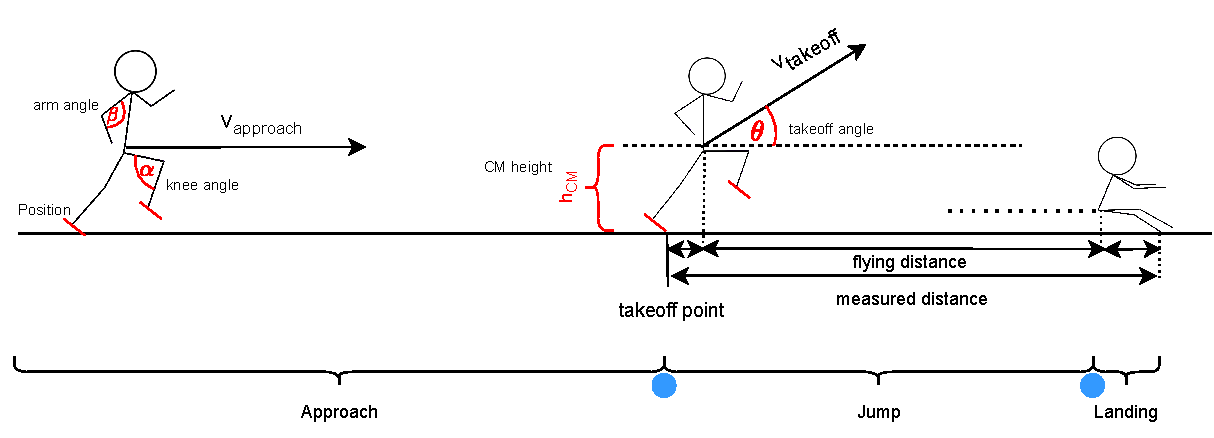
\includegraphics[scale=0.6]{long_jump_sketch.pdf}
    \caption[Long jump parameter overview]{General overview of the parameters
    that are important in a long jump.\\
    Parameters that can be analyzed by the software are marked
    \textcolor{red}{red}.\\
    The \textcolor{cyan}{blue points} indicate phase transition points.}
    \label{fig:4_long_jump_sketch}
\end{figure}
\FloatBarrier

\subsection{Detecting body key points}\label{subsec:4_body_keypoint_detection}

\subsection{Calculating analysis parameters}\label{subsec:4_calc_params}

\subsection{Automatic takeoff frame detection}\label{subsec:4_takeoff_detection}
Generally, a long jump can be divided into three different phases, namely
approach, jump and landing.
In \autoref{fig:4_long_jump_sketch} an overview over the phases is given,
where the takeoff phase is represented by the first phase changing point.\\
Each phase demands different requirements from an athlete, however, the
takeoff phase is the last phase in which an athlete is able to actively
influence the most important jumping conditions.
Within this short\footnote{0.1s \- 0.2s\cite{mechanical_power_long_jump}} time
period the initial kinetic run-up energy is transformed into jumping energy.
Especially the velocity vector of an athletes' \ac{CM} changes its direction
in the moment of the takeoff, as illustrated in
\autoref{fig:4_long_jump_sketch}.
The forces produced during the takeoff strongly influence the resulting
jumping distance. 
Thus, it is important to understand its dynamics.\\
Due to the short time period a takeoff takes, it can be difficult to detect
the takeoff frame in a long jump video in order to be able to analyze the
exact pre-jump conditions.\\\\
However, especially to allow for an on-field jumping analysis, a quick takeoff
frame detection is crucial.
Thus, an algorithm that can automatically detect the takeoff frame in a long
jump video is implemented in the following.\\\\
As the automatic takeoff frame detection is based on the parameters listed in
\autoref{sec:4_analysis_software}, the left and right
foot position as well as the position of the \ac{CM} were analyzed in
pre-recorded long jump videos of male long jumpers at different professional
levels reaching from hobby- to olympian athlete.
Moreover, the videos used differ in their length and quality as well as in the
jumping part they show (e.g.\ video 2 does not show the full run-up).
The results of three exemplary video analysis are shown in
\autoref{fig:4_angles_height_plot}.
In order to develop an accurate takeoff point detection, the takeoff frame was
first manually selected (marked as \textcolor{blue}{blue vertical line} for
each analysis in \autoref{fig:4_angles_height_plot}).\\
The presented data has not been cleaned up in any way.
This can especially be seen in the first and last analysis, in which the
position and angle data is not accurate due to body key point detection
inaccuracies.
These inaccuracies however are not of great interest as the key points are
detected correctly during the approach after a few frames.\\\\
In each analysis the left and right foot positions as well as the
according knee angles interchange from step to step.
The relative \ac{CM} height remains on the same level during the approach.\\
Behind the takeoff point, the relative hip- and foot heights increase quickly
until the maximal height is reached and the landing phase starts.
Moreover, the swing legs' foot height increases faster in comparison to the
jumping legs' foot height as the latter one stays on the ground longer to
introduce the jump.\\
In the moment of the takeoff, the knee angle of the jumping leg is above 170
degree, meaning the jumping leg is fully extended.
The swing legs' knee angle varies in the shown examples around 100 degree.\\\\
The visually most significant change which happens in the moment of the
takeoff and is therefore the most meaningful measured parameter that indicates
the takeoff is the change of height of the \ac{CM}.
Thus, the automatic takeoff detection is developed based on this parameter.\\
To approach the detection of the rapid change in the \ac{CM}s' vertical
velocity, a mathematical description of its position during the jump is
modelled.

\begin{figure}[h!]
    \begin{subfigure}[b]{0.5\textwidth}
        \includegraphics*[scale=0.45]{jump_runup_poor_start.png}
        \captionsetup{justification=centering, singlelinecheck=false, labelfont=bf}
        \label{subfig:runup_jump_landing_height}
    \end{subfigure}
    \begin{subfigure}[b]{0.5\textwidth}
        \includegraphics*[scale=0.45]{jump_runup_poor_start_angles.png}
        \label{subfig:runup_jump_landing_angles}
    \end{subfigure}
    \begin{subfigure}[b]{0.5\textwidth}
        \includegraphics*[scale=0.45]{jump_no_runup.png}
        \label{subfig:no_runup_height}
    \end{subfigure}
    \hfill
    \begin{subfigure}[b]{0.5\textwidth}
        \includegraphics*[scale=0.45]{jump_no_runup_angles.png}
        \label{subfig:no_runup_angles}
    \end{subfigure}
    \begin{subfigure}[b]{0.5\textwidth}
        \includegraphics*[scale=0.45]{jump_runup_poor.png}
        \label{subfig:runup_jump_height}
    \end{subfigure}
    \begin{subfigure}[b]{0.5\textwidth}
        \includegraphics*[scale=0.45]{jump_runup_poor_angles.png}
        \label{subfig:runup_jump_angles}
    \end{subfigure}
    \caption[Analyzed jumping parameters over time]{Analyzed and calculated
    jumping parameters over time.\\
    \textbf{Left column}: Analyzed left / right foot height and hip height.\\
    \textbf{Right column}: Calculated knee angles over time.\\
    The \textcolor{blue}{vertical lines} represent the visually selected
    takeoff point.\\
    \textbf{First row}: full run-up, full jump. \textbf{Second Row}: short 
    run-up, full jump.
    \textbf{Third row}: full run-up, full jump, poor video quality}
    \label{fig:4_angles_height_plot}
\end{figure}
\FloatBarrier

\subsubsection{Regression}
As the takeoff point detection is based on linear and quadratic regression,
both are briefly introduced in the following.
Regression generally describes the approximation of a polynomial function to
fit a given dataset.
The dataset that is tried to be approximated in this case is the height of the
\ac{CM}.
The dataset can be expressed as (T, H), where H holds the heights of the
\ac{CM} and T holds the related time points.
As the input is a video, T represents a simple vector holding the
video's frame numbers.
For the following steps it is helpful to express T and H as column vectors:
\begin{equation}
    \vec{t} = \begin{bmatrix}
        1\\
        2\\
        \vdots\\
        n
    \end{bmatrix}
        \quad\text{and}\quad
    \vec{h} = \begin{bmatrix}
        h_1\\
        h_2\\
        \vdots\\
        h_n
    \end{bmatrix}
\end{equation}
where n is the total number of video frames and $h_i$ is the $i\--th$ recorded
height of the \ac{CM}.\\
Taking the \ac{CM} in \autoref{fig:4_angles_height_plot} into consideration,
a whole jump can hardly be fitted with a single polynomial function.
However, as shown in \autoref{fig:4_long_jump_sketch}, a long jump consists of
multiple phases.\\
This offers an opportunity to detect the takeoff.
As mentioned before, the takeoff frame is defined as the point where the
approach phase ends and the jumping phase starts, ($PT_0$ in
\autoref{fig:4_long_jump_sketch}).
Thus, if a mathematical expression can be found for each phase respectively,
the takeoff frame is found implicitly.\\
The runup phase includes all frames in the interval $[0, PT_0[$, the jumping
phase is covered by the frames in range $[PT_0, PT_1[$ and the landing phase
is shown by the frames in the interval $[PT_1, n[$, where $PT_0$ defines the
first Phase Transition point (the takeoff) and $PT_1$ the point at which the
landing phase starts.
Each phase by itself can be approximated with a polynomial function.
The approach and the landing can be fitted using a linear expression.\\
Thus, two linear regressions are performed separately to find two expressions
of the form
\begin{equation}\label{eq:linear_function}
    \\y_i = \beta_0 + \beta_1t_i + \epsilon_i
    \quad\quad
    i = \text{start},\ \dots\ ,\text{end}
\end{equation}
where $\beta_0$ and $\beta_1$ are the coefficients that need to be found.
start and end represent the first and last frame index that should be
considered in the linear regression.
For the approach phase this leads to $start = 0$ and $end = TP_0 - 1$, the
landing phase is accordingly represented by $start = TP_1$ and $end = n - 1$.\\
\autoref{eq:linear_function} can also be expressed as matrix equation:
\begin{equation}\label{eq:linear_reg_matrix}
    \underbrace{
    \begin{bmatrix}
        y_0\\
        y_1\\
        \vdots\\
        y_r\\
    \end{bmatrix}}_{\substack{\vec{y}}}
    =
    \underbrace{
    \begin{bmatrix}
        1 & t_{\text{start}}\\
        1 & t_{\text{start} + 1}\\
        \vdots & \vdots\\
        1 & t_{\text{end}}
    \end{bmatrix}}_{\substack{\text{Design matrix} \\ T}}
    \underbrace{
    \begin{bmatrix}
        \beta_0\\
        \beta_1
    \end{bmatrix}}_{\substack{\text{Coefficients} \\ \text{vector} \\
    \vec{\beta}}}
    +
    \underbrace{
    \begin{bmatrix}
        \epsilon_0\\
        \epsilon_1
    \end{bmatrix}}_{\substack{\text{Error} \\ \text{vector} \\
    \vec{\epsilon}}}
\end{equation}
where $r = end - start$.
This can be written in short form as:
\[
    \vec{y} = T\vec{\beta} + \vec{\epsilon}    
\]
Now, the vector $\vec{\beta}$ needs to be found that minimizes the sum of
errors $E_{SSE}$ between the measured \ac{CM} height $h_i \in \vec{h}$ and the
fitted polynomial $y_i$ at time step i.
To measure the error, the \ac{SSE} is used:
\begin{equation}
    E_{SSE} = \sum_{i=start}^{end} \epsilon_i^2 = \sum_{i=start}^{end} (h_i - y_i)^2
\end{equation}
Using the simple linear expression from \autoref{eq:linear_function},
following error function is found:
\begin{equation}
    E_{SSE} = \sum_{i=start}^{end} (h_i - \beta_0 - \beta_1i)^2
\end{equation}
By using the matrix notation introduced in \autoref{eq:linear_reg_matrix},
the equation above can be written in matrix notation as well:
\begin{equation}\label{eq:sse_matrix}
    E_{SSE} = (T\vec{\beta} - \vec{h})^T(T\vec{\beta} - \vec{h})
\end{equation}
As $\vec{\beta}$ should minimize $E_{SSE}$, the minimum of $E_{SSE}$ is
needed, which can be found by solving following equation:
\begin{equation}\label{eq:gradient_linear_case}
    \nabla_{\vec{\beta}}E_{SSE} = \nabla_{\vec{\beta}}(T\vec{\beta} - \vec{h})^T(T\vec{\beta} - \vec{h}) = 0
\end{equation}
where $\nabla_{\vec{\beta}}$ denotes the gradient with respect to $\vec{\beta}$.\\
The coefficients can then easily be found by solving
\autoref{eq:gradient_linear_case} for $\vec{\beta}$, which yields the 
following normal equation:
\begin{equation}\label{eq:normal_equation}
    \vec{\beta} = (T^T T)^{-1}(T^T\vec{h})
\end{equation}
that especially requires $(T^{T} T)$ to be invertible.
A proof of \autoref{eq:normal_equation} can be found in
\cite{proof_linear_regression_mat}.\\
As mentioned, this process is performed twice to find a linear approximation
for the approach and the landing phase of an athletes' \ac{CM} respectively.\\\\
The jumping phase cannot be approximated with a linear polynomial.
However, as can be seen in \autoref{fig:4_angles_height_plot} after the marked
takeoff point, the curve of the \ac{CM} height can be approximated using a
parabola.
Thus, quadratic regression is used to find a curve that describes the height
of the \ac{CM} during the jumping phase.
The second order polynomial that needs to be found is of the form:
\begin{equation}\label{eq:quadratic_function}
    \\y_i = \beta_0 + \beta_1t_i + \beta_2t_i^2 + \epsilon_i
    \quad\quad
    i = PT_0,\ \dots\ ,PT_1 - 1
\end{equation}
$PT_0\ \text{and}\ PT_1$ are the phase transition points shown in
\autoref{fig:4_long_jump_sketch}.
The following steps are equal to the linear regression shown above.
Thus, only the differences are shown in detail.\\
The T matrix in \autoref{eq:linear_reg_matrix} contains all frame
numbers as column vector.
Because a linear relation was tried to be found to approximate the approach
and  landing phase before, the T matrix as well only contained linear values.
Now however, a quadratic relation needs to be found.
Thus, the T matrix needs to be extended by one more column holding the
quadratic frame numbers yielding following matrix equation:
\begin{equation}\label{eq:quadratic_reg_matrix}
    \underbrace{
    \begin{bmatrix}
        y_0\\
        y_1\\
        \vdots\\
        y_r\\
    \end{bmatrix}}_{\vec{y}}
    =
    \underbrace{
    \begin{bmatrix}
        1 & t_{PT_0} & t_{PT_0}^2\\
        1 & t_{PT_0 + 1} & t_{PT_0 + 1}^2\\
        \vdots & \vdots & \vdots\\
        1 & t_{PT_1 - 1} & t_{PT_1 - 1}^2
    \end{bmatrix}}_{T}
    \underbrace{
    \begin{bmatrix}
        \beta_0\\
        \beta_1\\
        \beta_2
    \end{bmatrix}}_{\vec{\beta}}
    +
    \underbrace{
    \begin{bmatrix}
        \epsilon_0\\
        \epsilon_1\\
        \epsilon_2
    \end{bmatrix}}_{\vec{\epsilon}}
\end{equation}
where $r = PT_1 - 1 - PT_0$.
The error function which needs to be minimized can be set equivalent to the
linear case (\autoref{eq:sse_matrix}).
Comparing \autoref{eq:linear_reg_matrix} and \autoref{eq:quadratic_reg_matrix}
the only things that change are the number of coefficients (and thus the
number of error terms) as well as the design matrix T, which holds one more
column.
The steps to determine the coefficients $\vec{\beta}$ are equal to the linear
case in equations~\ref{eq:sse_matrix} to~\ref{eq:normal_equation}.
$\vec{\beta}$ is then given by the same normal equation~
\ref{eq:normal_equation} as in the linear case:
\[
    \vec{\beta} = (T^T T)^{-1}(T^T\vec{h}) 
\] 
where $\vec{\beta}$ contains three coefficients $\beta_0$, $\beta_1$ and
$\beta_2$ to approximate the jumping phase.\\\\

\noindent By using this linear- and quadratic regression approach, the whole
jump can be modelled mathematically.
However, in order to find the best fitting model, the phase changing points
($PT_0$ and $PT_1$ in \autoref{fig:4_long_jump_sketch}) need to be determined.
This can be done by minimizing the overall error $E_{total}$, which is defined
as the sum of regression errors resulting from the three independent
regressions performed (one per jumping phase):

\begin{equation}
    E_{total} = E_{approach} + E_{jump} + E_{landing}
\end{equation}

\noindent $E_{total}$ can be minimized by using a brute-force approach.
For each possible combination of phase transition points, two linear
regressions (representing approach and landing) and one quadratic regression
(representing the jumping phase) are performed and their individual errors
given by \autoref{eq:sse_matrix} are summed up.
The combination of phase transition points that leads to the minimal
$E_{total}$ is then considered as the optimal model to fit the overall jump.
As the found phase transition points directly represent their corresponding
frame numbers, the takeoff frame is directly given by the first phase
transition point.\\

\begin{figure}[htp]% [H] is so declass\'e!
    \centering
    \begin{minipage}{0.45\textwidth}
    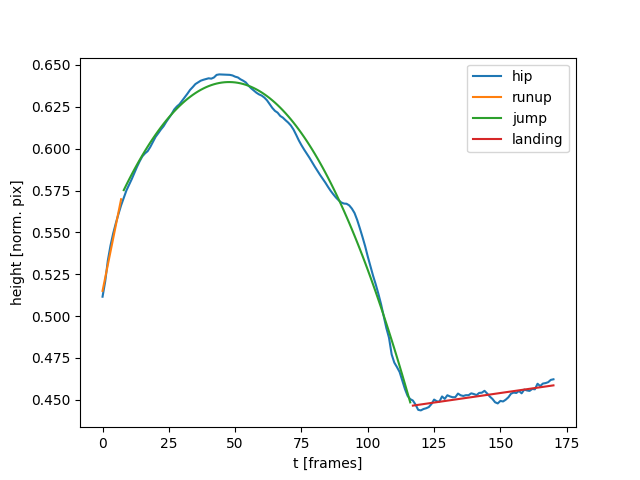
\includegraphics[width=\textwidth]{regression_jump_only.png}
    \caption{figure caption}
    \end{minipage}\hfill
    \begin{minipage}{0.45\textwidth}
    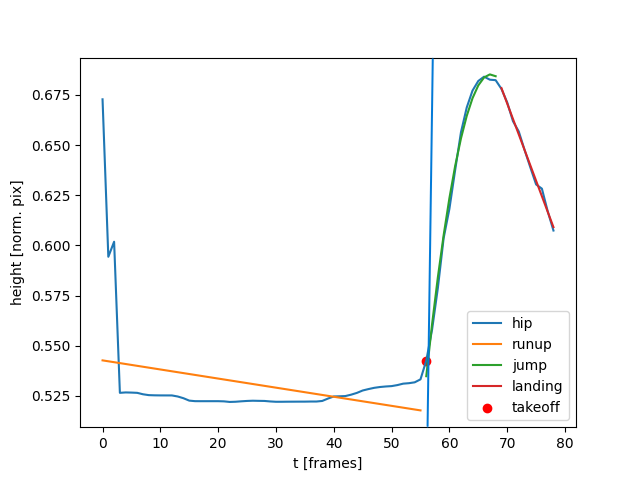
\includegraphics[width=\textwidth]{regression_poor_approach.png}
    \caption{figure caption}
    \end{minipage}\par
    \vskip\floatsep% normal separation between figures
    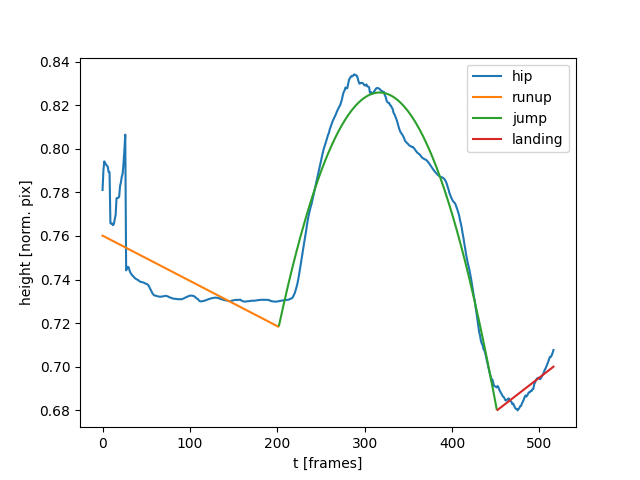
\includegraphics[width=0.45\textwidth]{regression_poor_approach_jump.png}
    \caption{figure caption}
    \end{figure}
\FloatBarrier

\begin{algorithm}
    \caption{takeoff\_frame(hip\_height: array)}
    \begin{algorithmic}[1]
    \State $n \gets \text{length of } hip\_height$
    \State $total\_error \gets 100$
    \State $changing\_points \gets (0,0)$
    \State $runup\_coeffs \gets []$
    \State $jump\_coeffs \gets []$
    \For{$i \gets 0$ \textbf{to} $n - 2$}
        \For{$j \gets i + 2$ \textbf{to} $n$}
            \State $x\_runup \gets \text{array of } i \text{ elements from } 0 \text{ to } i - 1$
            \State $x\_jump \gets \text{array of } (j - i) \text{ elements from } 0 \text{ to } j - i - 1$
            \State $x\_landing \gets \text{array of } (n - j) \text{ elements from } 0 \text{ to } n - j - 1$
            \State $hip\_fit\_runup, residuals\_runup \gets \text{polyfit}(x\_runup, hip\_height[:i], 1)$
            \State $hip\_fit\_jump, residuals\_jump \gets \text{polyfit}(x\_jump, hip\_height[i:j], 2)$
            \State $hip\_fit\_landing, residuals\_landing \gets \text{polyfit}(x\_landing, hip\_height[j:], 1)$
            \State $fitting\_error \gets residuals\_runup + residuals\_jump + residuals\_landing$
            \If{fitting\_error $<$ total\_error \textbf{and} hip\_fit\_jump[0] $<$ 0}
                \State $total\_error \gets$ fitting\_error
                \State $changing\_points \gets (i,j)$
                \State $runup\_coeffs \gets hip\_fit\_runup$
                \State $jump\_coeffs \gets hip\_fit\_jump$
            \EndIf
        \EndFor
    \EndFor
    \State \textbf{return} changing\_points
    \end{algorithmic}
    \end{algorithm}

\section{Hardware setup}\label{sec:4_hardware}
In order to capture high-quality video recordings that cover a complete long 
jump, from the first step all the way to the landing, a drone is used to fly
next to the athlete throughout the whole process.
Thus, a drone in form of a quadcopter is built from scratch.
Its control will be integrated seamlessly in the projects' \ac{GUI}.\\
This section introduces the hardware components that are used for building 
this drone as well as its flight control unit.\\
A short outline of the hardware is given in 
\autoref{subsec:4_hardware_selection},
while \autoref{subsec:4_hw_setup} focuses on the overall assembly of the 
selected hardware.

\subsection{Hardware selection}\label{subsec:4_hardware_selection}
Currently, commercial drone hardware on the market is mainly separable into 
the two large areas of fully remote controlled \ac{FPV} hardware and hardware 
for (autonomous) drones that can usually carry more load, e.g.~heavy cameras.
Even though the quadcopter in this project needs to be remotely 
controllable from a ground station pc, it is still more likely to be located 
in the latter one.\\
Generally the hardware was chosen based on the following criteria:
\begin{itemize}
    \item price
    \item compatibility
    \item size
\end{itemize}

\subsection*{Flight Hardware}\label{subsec:4_filght_hardware}
The main hardware that a quadcopter needs to fly will, in the following, be
referred to as \textit{flight hardware}.
This includes frame, motors, rotors, \acp{ESC} and a \ac{PDB}.\\
The main platform on which all drone hardware is mounted, is referred to as
a quadcopter's frame.
As this project's drone does not need to carry any heavy load, such as high 
precision camera systems or other sensors, a rather compact frame would 
theoretically be sufficient.
However, compact frames tend to be less stable compared to larger frame sizes 
which could lead to a lower video recording quality and thus require more 
complex post-processing software.
Moreover, the assembly process on larger frames is more convenient and 
replacing parts is easier.
Additionally, compact frames are most commonly used in areas that demand quick
reaction times for high speed flight maneuvers, e.g.~in drone racing.
This however is not needed in this project's context.\\
Taken the mentioned considerations into account the mid-sizes \textit{Holybro 
S500 V2} frame kit is chosen.
Besides the frame, the kit also includes a landing gear and rotors.
Moreover, the main platform includes a \ac{PDB} to split the battery's power 
equally to all four motors.\\
An overview of all included parts is given in \autoref{fig:4_frame_kit}.
\begin{figure}[!h]
    \centering
    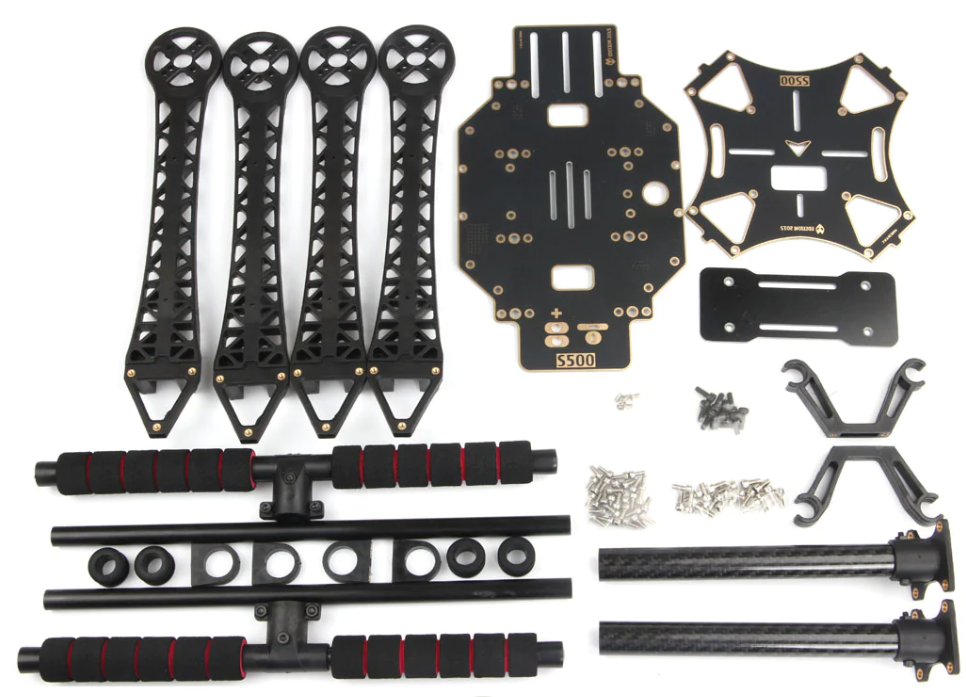
\includegraphics[scale=0.6]{frame-kit.png}
    \caption[Frame kit]{Holybro S500 V2 frame kit}
    \label{fig:4_frame_kit}
\end{figure}
\FloatBarrier
\noindent Besides the frame, motors and compatible \acp{ESC} are crucial 
flight hardware components.
Each motor requires an own \ac{ESC} that translates signals from a flight 
control unit to a voltage and thereby control the motors' rotation speed.
To guarantee compatibility, both components were chosen from Holybro as well
and can be seen in \autoref{fig:motors_and_esc}.
\begin{figure}[!h]
    \begin{subfigure}[b]{0.48\textwidth}
        \includegraphics*[scale=0.15]{motor.jpg}
        \caption{920KV Motor}
        \label{subfig:motor_picture}
    \end{subfigure}
    \hfill
    \begin{subfigure}[b]{0.5\textwidth}
        \includegraphics*[scale=0.15]{esc.jpg}
        \caption{\acl*{ESC}}
        \label{subfig:esc_picture}
    \end{subfigure}
    \caption[Motor and \acs*{ESC}]{Motor (a) and \acs*{ESC} (b)}
    \label{fig:motors_and_esc}
\end{figure}
\FloatBarrier
The drones' motors performance capabilities are defined by the number of 
\ac{RPM} they can perform per 1V input.
As can be seen in \autoref{subfig:motor_picture}, this link between 
rotation speed and input voltage is expressed in the arbitrary unit \textit{KV}.
The chosen motors are capable of rotating with a speed of 920~\ac{RPM} per 1V 
input voltage. 
Put into context, this is a common rotation speed in commercial and hobby 
drone applications.
Racing drones however, operate at motor speeds of up to 3500~KV.

\subsection*{Control Hardware}\label{subsec:4_control_hardware}
In order to perform flight maneuvers with a quadcopter, each motor must be
controllable individually.
The calculation of the correct rotation speeds is generally performed by 
a \textit{flight control unit}.
Usually, it receives directional instructions from a remote control as input,
combines them with many parameters (e.g.~\acs{GPS} position, height over ground,
speed, etc.) and generates a (\acs{PWM}) output signal for each motor.\\
Within this project the flight controller needs to deal with two different 
inputs.
First, the ground station which can be seen as a remote control in this case.
Additionally, the drone should be able to fly autonomously next to an athlete
during their long jump training.
Here, the second input gets important.
The autonomous fly option requires the quadcopter to perform a person 
detection and therefore image processing on-board.
As the flight controller itself is not able to perform such calculations, an
additional \textit{companion computer} is required.
This companion computer will then send directional instructions just like the 
ones from the ground station to the flight controller and thereby control the 
drone.\\
The combination of flight controller and on-board companion computer will in 
the following be called \textit{control hardware}.\\
There are many types of different flight controllers available commercially.
However, most of them are not meant to be used in combination with a companion
computer.\\
Two of the most commonly used flight controllers in autonomous drone projects
are the \textit{PixHawk} and the \textit{Navio2}.
They are often chosen because they both work together seamlessly with a 
companion computer.
The former is a totally independent system which can also operate without any 
supporting computer.
The latter is implemented as \ac{HAT} specifically designed for a Raspberry 
Pi.
Thus, it does not include an own \ac{CPU} but uses the Raspberry Pis's 
resources to perform flight relevant calculations.\\
A detailed comparison between both flight controllers is given in 
\autoref{table:4_flight_cotroller_cmp}.
\begin{table}[h!]
\centering
\begin{tabular}[c]{|p{4cm}||p{4cm}|p{4cm}|}
\hline
\multicolumn{3}{|c|}{Flight Controller Comparison}\\
\hline
Criteria & PixHawk & Navio2\\
\hline
\hline
Processor & ARM Cortex M4 with FPU / 32-bit co-processor & Depends on Raspberry
Pi version\\
\hline
Sensors & ST Micro 16-bti gyroscope, ST Micro 14-bit accelerometer, MEAS
barometer & MPU9250 9DOF IMU, LSM9DS1 9DOF IMU, MS5611 Barometer, U-blox M8N 
Glonass/\acs{GPS}/Beidou\\
\hline
Interfaces & UART, Spektrum DSM, PPM / S.BUS input, I2C, SPI, CAN, USB, 3.3V 
and 6.6V ADC input, 8 \acs{PWM} outputs, 6 Auxiliary outputs & UART, I2C, ADC, PPM / 
S.BUS input, 14 \acs{PWM} outputs\\
\hline
Dimensions\newline(W x H x L) in mm & $50 \times 15.5 \times 81.5$ & $55 \times 65$\\ 
\hline
Other & Failsafe options (e.g. extra power supply, \acs{GPS}, etc.) & None\\
\hline
Price (Eur.) & TBD & TBD\\
\hline
\end{tabular}
\caption[Flight controller comparison]{Comparison between PixHawk and 
Navio2 flight controller.}
\label{table:4_flight_cotroller_cmp}
\end{table}

\noindent As can be seen, both flight controllers offer different interfaces 
to connect additional hardware.
Moreover, both systems include sensors, mostly to gather information about 
drone's current position and inertia.
Here, the Navio2 even offers more sensors, as it already includes a \ac{GPS} 
sensor, while the PixHawk relies on an external one.\\\\
\noindent For this project, the PixHawk was chosen over the Navio2 mainly for 
three reasons.
First, it is on the market for a long time already and thus have a large 
community support.
Secondly, as it is an independent system, a failure of the companion computer 
will not lead to a crash.
Lastly, it allows for a wide range of companion computers, while the Navio2 
can only interoperate with a Raspberry Pi.\\
Furthermore, the mentioned considerations lead to easy rapid prototyping 
approaches, as the drone can be manually flown without a companion computer in
a first implementation.

\subsection{Hardware assembly}\label{subsec:4_hw_setup}
In the following, a high-level overview of the quadcopters' hardware setup is 
given.
The general wiring is shown and explained before a short introduction of some 
important communication protocols is given.

\subsection*{General wiring}
In the following \autoref{fig:4_general_wiring} the general wiring layout is 
shown.
The whole system is powered from one power source only.
\begin{figure}[!h]
    \centering
    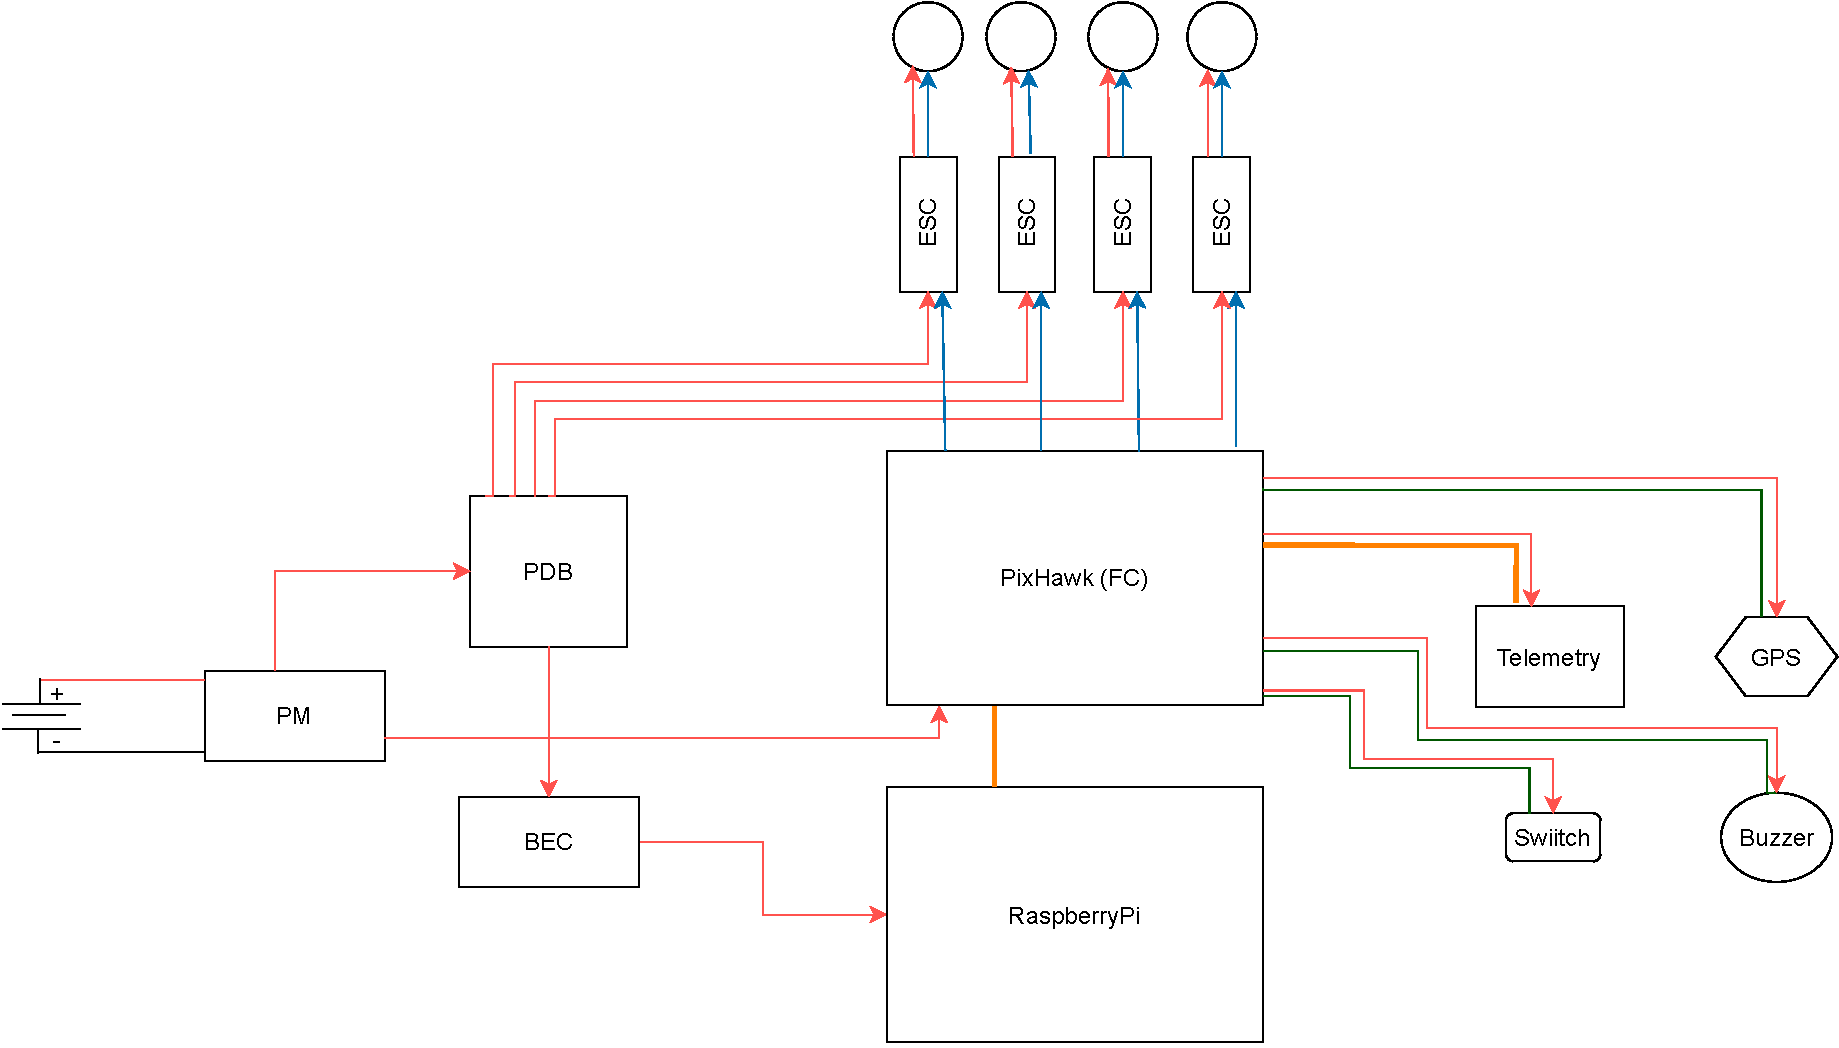
\includegraphics[scale=0.5]{general_wiring.pdf}
    \caption[General Wiring]{General wiring of the hardware setup.\\
    Power connections are labeled red, 
    Blue connections are used for \ac{PWM} signals, 
    Green connections are serial connections, 
    orange connections are more specifically serial UART connections.}
    \label{fig:4_general_wiring}
\end{figure}
\FloatBarrier
\noindent This results in some challenges in providing the correct voltage for
each connected device.
In the current setup this task is taken over by three devices.
The \ac{PM} is directly connected to the battery.
It transfers the battery's voltage to the \ac{PDB} and a lower 5V voltage to
the PixHawk flight controller.
The \ac{PDB} itself is a parallel circuit, thus providing the same voltage
(battery voltage) to each output.
The third device is a \ac{BEC} which is directly connected
to the \ac{PDB} and delivers a constant 5V output.
This can be used to power a companion computer such as a RaspberryPi.\\
All other required peripherals are powered by the PixHawk flight controller
itself.
The main peripherals used in this project are a telemetry module which is used
for communication with a ground station and a \ac{GPS} module used for
improving the drones capabilities to follow a defined trajectory, which is
specifically useful for auto-return~and landing features.
Two more peripherals, a buzzer to output audio warning signals and a manual
kill switch which can immediately stop all four motors, are installed mainly
for safety reasons.\\
The hardware components that actually control the motor rotation speeds,
the \acp{ESC}, are connected to the \ac{PDB} for power supply as well as to
the flight controller that calculates the correct rotation speeds based on the
wanted flight maneuvers and outputs a \ac{PWM} signal for each motor.\\
The presented overall wiring is rather complex but allows relying on one power
source only instead of using multiple power sources for flight hardware and
control hardware including peripherals respectively.

\subsection*{Communication between components}\label{subsec:4_comm}
The drone setup needs hardware components to communicate with each other in 
order to transfer control signals from either the companion computer or from
the ground station to the flight controller.
Even if both options origin from different sources, they use the same
device-to-device communication protocol.
The protocol used for this purpose is the \textit{UART} protocol, which is
acronym for universal asynchronous receiver / transmitter protocol.
It is based on a serial, full duplex connection using six connections.
The connection layout is shown in \autoref{fig:4_uart_wiring},
\begin{figure}[!h]
    \centering
    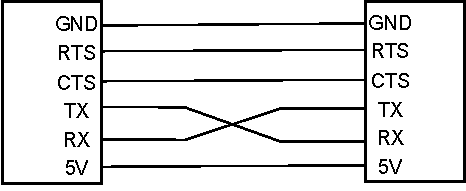
\includegraphics[scale=0.8]{uart_wiring.pdf}
    \caption[UART wiring]{UART wiring}
    \label{fig:4_uart_wiring}
\end{figure}
\FloatBarrier
\noindent where RTS / CTS denote Ready to send and Clear to send.
RX / TX represent the actual data receiving and sending connections
respectively.\\

\noindent UART transfers data using data frames with minimal overhead.
A typical UART frame consists of just a start bit, data bits, a parity bit and
a stop bit.
\autoref{fig:4_uart_frame} visualizes such a data frame. 
\begin{figure}[!h]
    \centering
    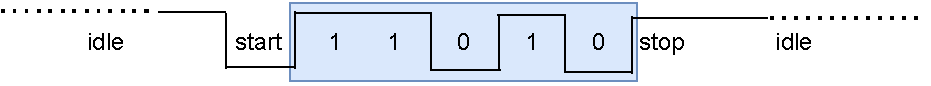
\includegraphics[scale=0.8]{uart_frame.pdf}
    \caption[UART data frame]{Exmple of an UART data frame. The blue marked
    area is the actual data part that is transmitted.}
    \label{fig:4_uart_frame}
\end{figure}
\FloatBarrier
\noindent The shown UART data frame includes 5 data bits, however, the amount
can vary between 5 and 9.
Moreover, the included even parity bit is optional.
The idle state is set to a voltage that represents HIGH level on purpose, so
that any connection failure is easily detectable.
UART can work with any voltages to denote HIGH and LOW levels.
In the quadcopter setup HIGH is represented by 5V and LOW by GND.
